\documentclass[aspectratio=169]{beamer}
%\usetheme{CambridgeUS}
%\usecolortheme{beaver}

%\usefonttheme{serif}
%\usepackage{helvet}

\usefonttheme{serif}     % Font theme: serif
%\usepackage{ccfonts}     % Font family: Concrete Math
\usepackage[T1]{fontenc} % Font encoding: T1

\setbeamersize{text margin left=42pt,text margin right=42pt} 
\setbeamertemplate{navigation symbols}{}
\setbeamertemplate{itemize items}[default]

\beamertemplatenavigationsymbolsempty

\definecolor{fore}{RGB}{51,51,51}
\definecolor{back}{RGB}{255, 254, 250}
\definecolor{title}{RGB}{ 255, 15, 0}
\definecolor{links}{RGB}{18, 168, 255}

\setbeamercolor{titlelike}{fg=title}
\setbeamercolor{normal text}{fg=fore,bg=back}
\setbeamercolor{alerted text}{fg=title}
\setbeamercolor{itemize item}{fg=title}
\setbeamercolor{enumerate item}{fg=title}
\hypersetup{colorlinks,urlcolor=links}

% for code https://kbroman.org/blog/2013/10/07/better-looking-latexbeamer-slides/
\usepackage{listings}
\definecolor{keywords}{RGB}{255,0,90}
\definecolor{comments}{RGB}{60,179,113}
\lstset{language=Python,
keywordstyle=color{keywords},
commentstyle=color{comments}emph}

% fonts
\usepackage[sc]{mathpazo}


% title info
\title{\textbf{Health and Equity}
\subtitle{\textbf{GGR424 - Transportation Geography \& Planning}}
\author{Jeff Allen}
\institute{University of Toronto}
\date{March 7, 2022}}




\begin{document}
	
\begin{frame}
	\titlepage	
\end{frame}





\begin{frame}
	
	\textbf{Announcements}
	
	\begin{itemize}
		\item Project Proposal due March 10
	\end{itemize}
	
	
	\textbf{Today}
	
	\begin{itemize}
		\item Health impacts of	transportation (e.g. pollution, noise, physical activity)
		\item How the costs and benefits of transportation are (in)equitably distributed
		
	\end{itemize}
\end{frame}




\begin{frame}
	
	How can urban transportation affect your health and well-being?
	
\end{frame}



\begin{frame}
	
	\textbf{Noise}
	
	\begin{figure}
		\centering
		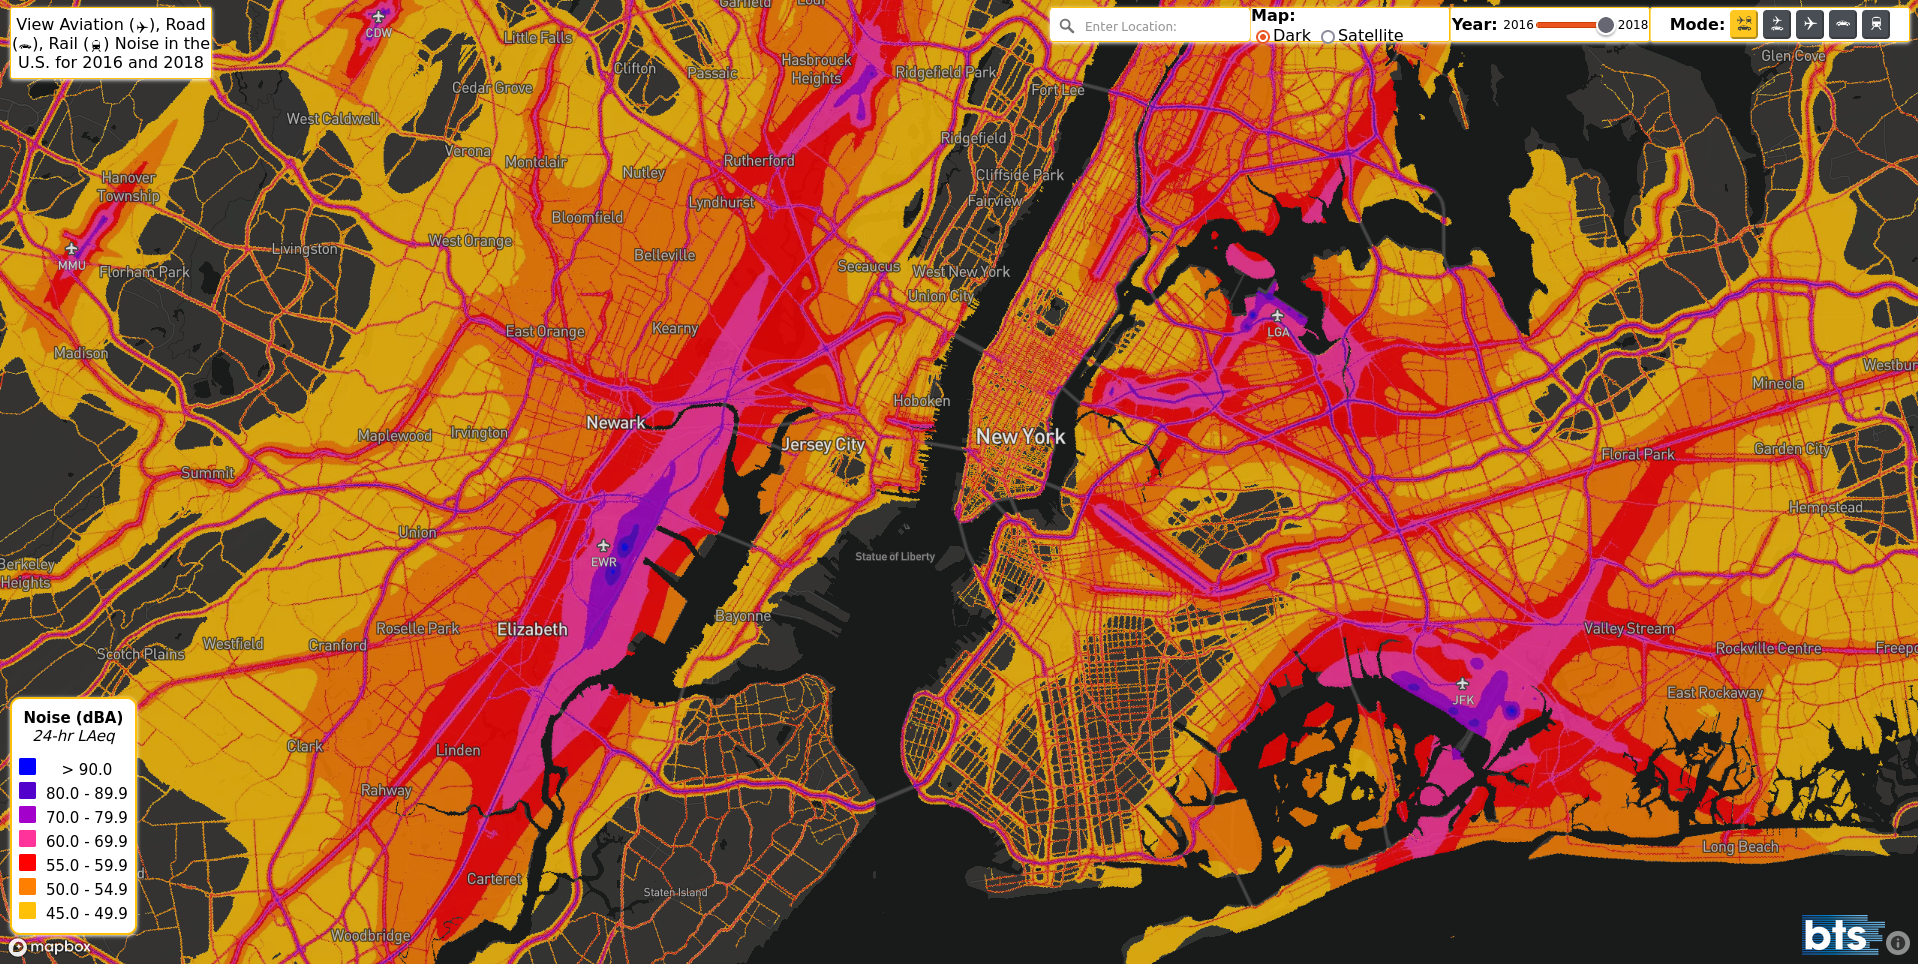
\includegraphics[width=1\linewidth]{images/noise_nyc.png}
	\end{figure}
	\tiny Source: \url{https://maps.dot.gov/BTS/NationalTransportationNoiseMap/}
	
	\vspace{2mm}
	\tiny City report on health impacts of noise \url{https://www.toronto.ca/wp-content/uploads/2017/11/8f98-tph-How-Loud-is-Too-Loud-Health-Impacts-Environmental-Noise.pdf}
	
\end{frame}

% annoyance, innability to concentrate (work school), loss of sleep, increased stress, increased risk of cardiovascular disease






\begin{frame}
	
	\textbf{Air Pollution}
	
	\begin{columns}
		\begin{column}{0.5\textwidth}
			
			
			\begin{figure}
				\centering
				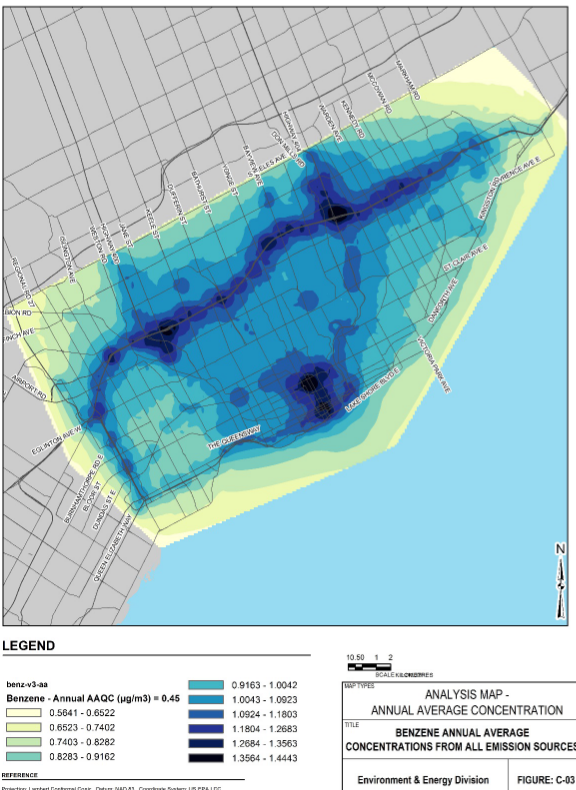
\includegraphics[width=0.8\linewidth]{images/tor_benzene.png}
			\end{figure}
		\end{column}
		
		\begin{column}{0.5\textwidth}
			\begin{figure}
				\centering
				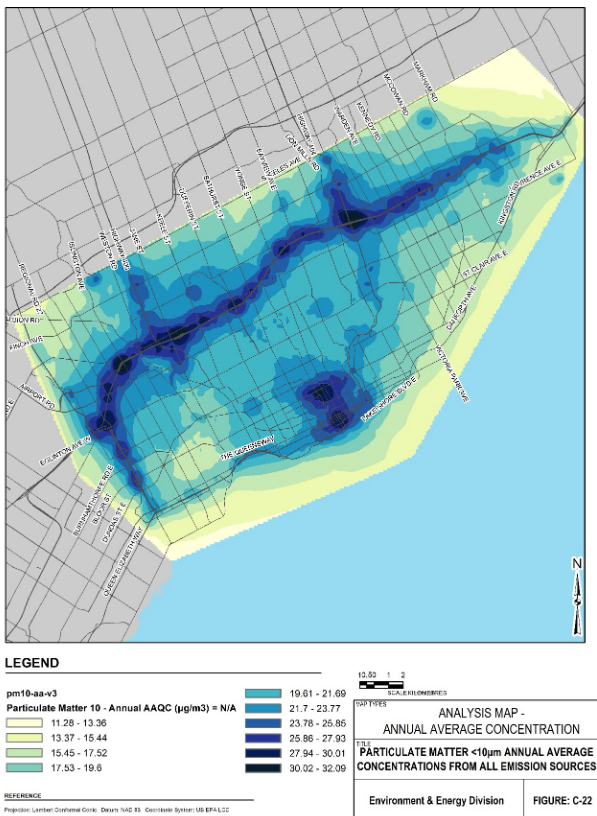
\includegraphics[width=0.8\linewidth]{images/tor_pm10.png}
			\end{figure}
			
		\end{column}

	\end{columns}
	
	\tiny City of Toronto. Avoiding the TRAP: Traffic-Related Air Pollution in Toronto and Options
	for Reducing Exposure. Technical Report. October 2017.: \url{https://www.toronto.ca/legdocs/mmis/2017/hl/bgrd/backgroundfile-108070.pdf}
	
\end{frame}


% pollution - e.g. missed days of activity (i.e. stay inside), asthma, bronchitus, hospitalizations/mortality, etc.






\begin{frame}
	\textbf{Active Travel and Physical Health}
	
	\begin{figure}
		\centering
		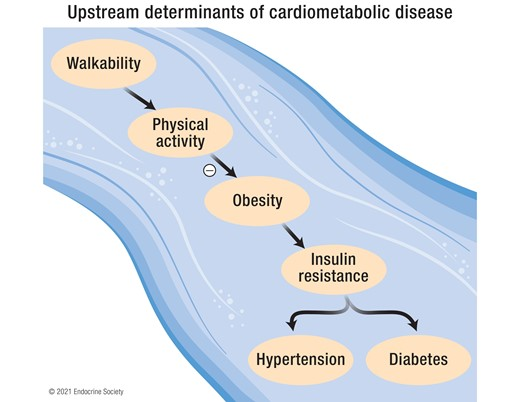
\includegraphics[width=0.6\linewidth]{images/walkability_health}
	\end{figure}
	
	\tiny The weight of place: Built environment correlates of obesity and diabetes \url{https://doi.org/10.1210/endrev/bnac005}
	
\end{frame}

% walkability and physical activity

\begin{frame}
	
	\begin{figure}
		\centering
		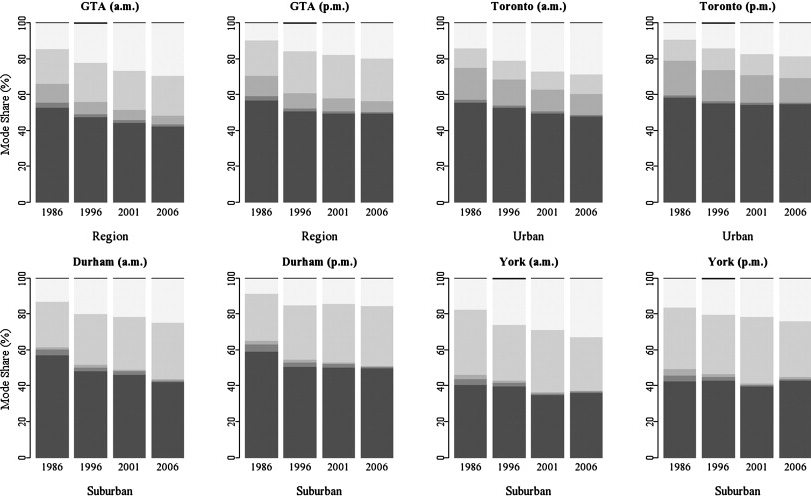
\includegraphics[width=0.9\linewidth]{images/mode_to_school}
	\end{figure}
	
	
	\tiny School travel mode share (\% of trips) by jurisdiction and year (children and youth, 11–13 years of age) in the Greater Toronto Area, Canada (1986–2006).
	
	\tiny\url{https://doi.org/10.1016/j.ypmed.2009.03.001}
	
\end{frame}






\begin{frame}
	
	\textbf{Satisfaction of travel}
	
	\begin{figure}
		\centering
		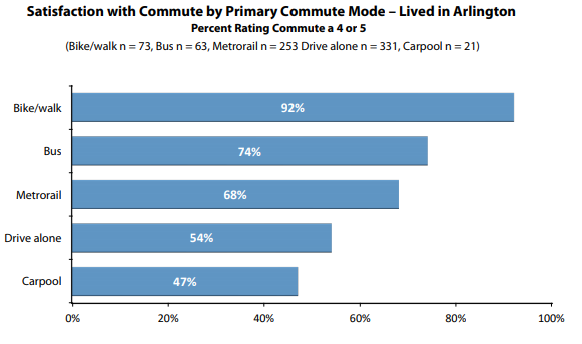
\includegraphics[width=0.7\linewidth]{images/mode_satisfaction.png}
	\end{figure}
	
	\tiny\url{https://mobilitylab.org/2020/09/29/the-pursuit-of-happiness-how-commute-mode-affects-commute-mood/}
	
\end{frame}

% stress of travel, long commutes means less time doing other things


\begin{frame}
	
	\textbf{Long commutes}
	
	\vspace{4mm}
	
	From the 2016 Canadian census:
	
	\begin{itemize}
		\item 9.7\% have a commute greater than 60 minutes
		
		\item 3.5\% have a commute greater than 75 minutes
		
		\item 2.5\% have a commute greater than 90 minutes
	\end{itemize}
	
\end{frame}




\begin{frame}
	
	Donald Appleyard’s
	“Livable Streets” was
	one of the first studies
	to look at the impact of
	traffic on social
	characteristics of
	streets
	
	\begin{figure}
		\centering
		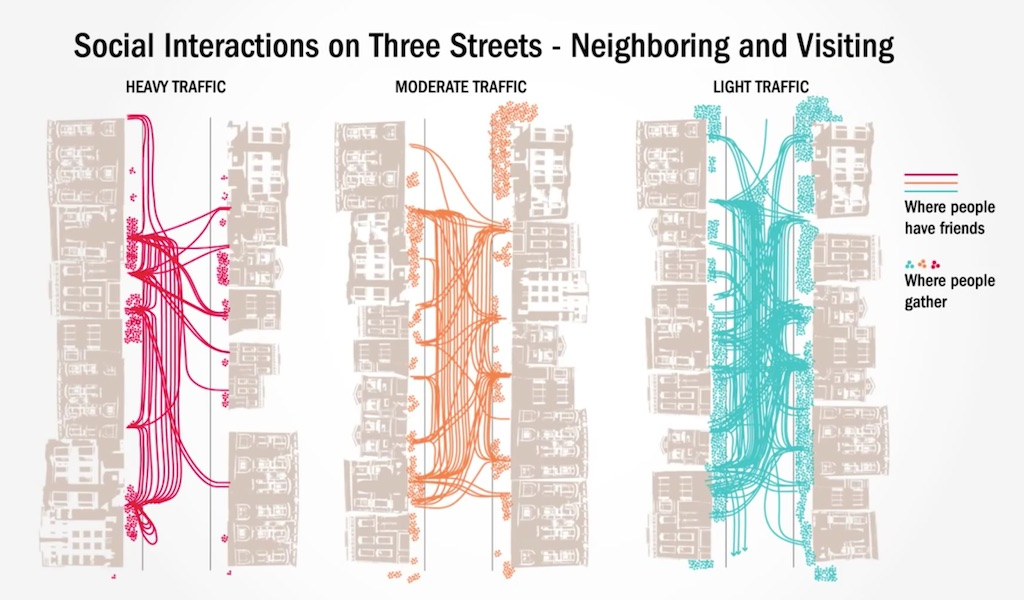
\includegraphics[width=0.94\linewidth]{images/Livable-Streets-Donald-Appleyard.jpg}
	\end{figure}
	
\end{frame}






% accidents, cars, pedestrians, etc. - but general feelings of safety


\begin{frame}
	
	\textbf{Safety, e.g. Collisions}
	
	\begin{figure}
		\centering
		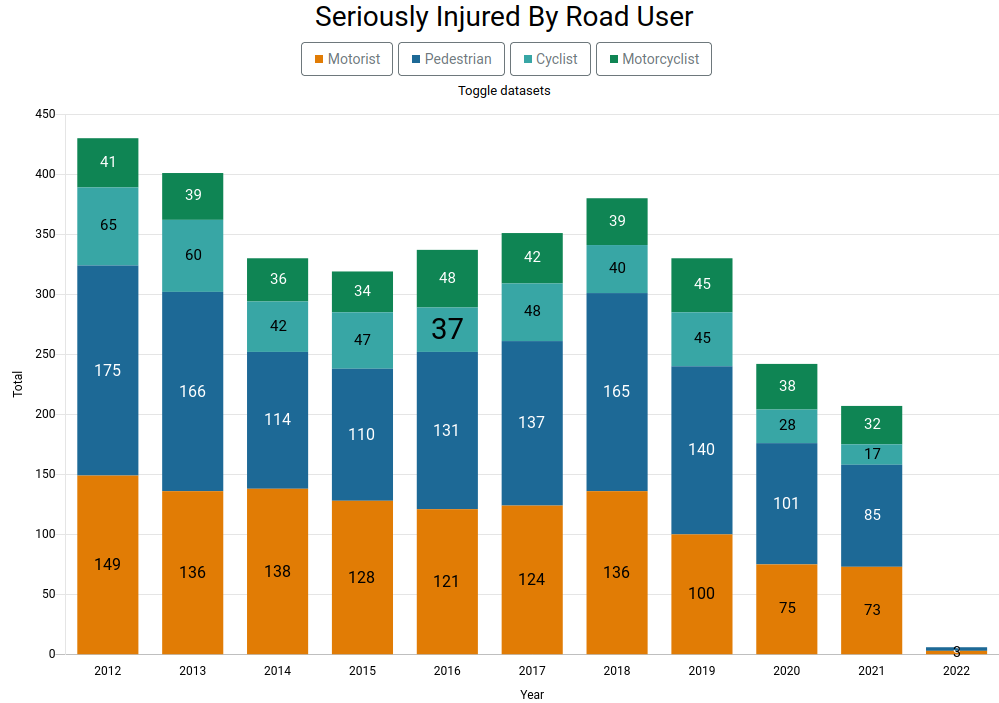
\includegraphics[width=0.7\linewidth]{images/injury_road_tor.png}
	\end{figure}
	
	\tiny \url{https://www.toronto.ca/services-payments/streets-parking-transportation/road-safety/vision-zero/vision-zero-dashboard/seriously-injured-vision-zero/}s
	
\end{frame}




\begin{frame}
	
	\textbf{Safety, e.g. COVID-19}
	
	\begin{figure}
		\centering
		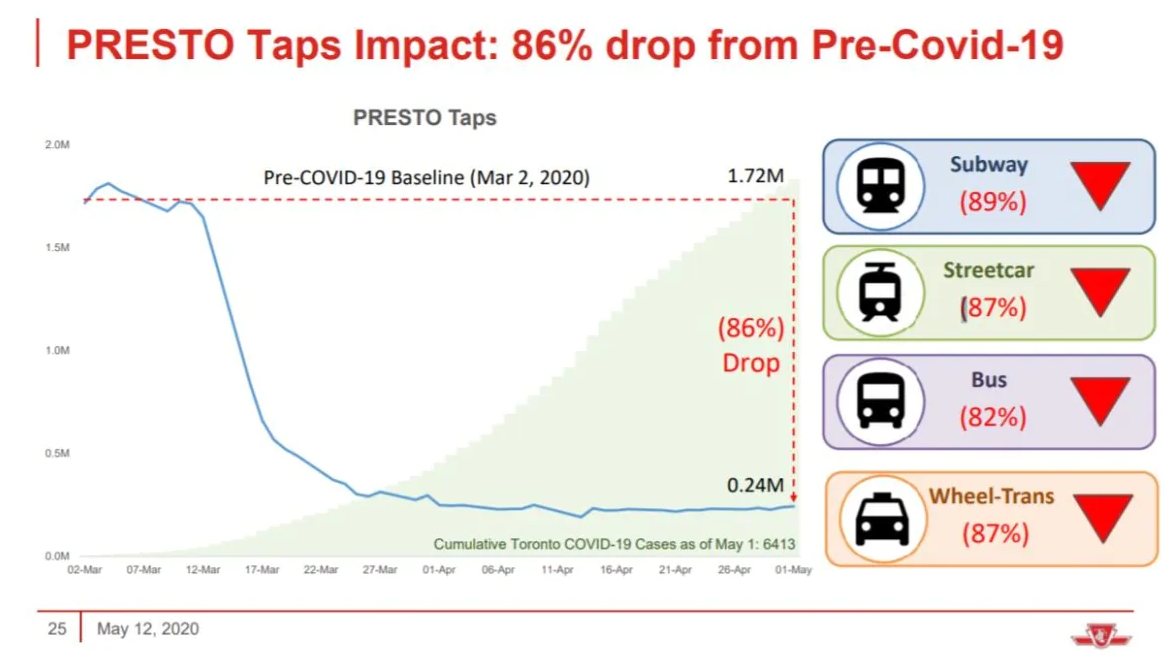
\includegraphics[width=0.94\linewidth]{images/ttc-covid.png}
	\end{figure}
	
		\tiny \url{https://www.cbc.ca/news/canada/toronto/ttc-finances-covid19-1.5569867}
	
\end{frame}




% access to health, groceries, etc. foodbanks

\begin{frame}
	
	\textbf{Accessibility, e.g. to healthy food}
	
	\begin{figure}
		\centering
		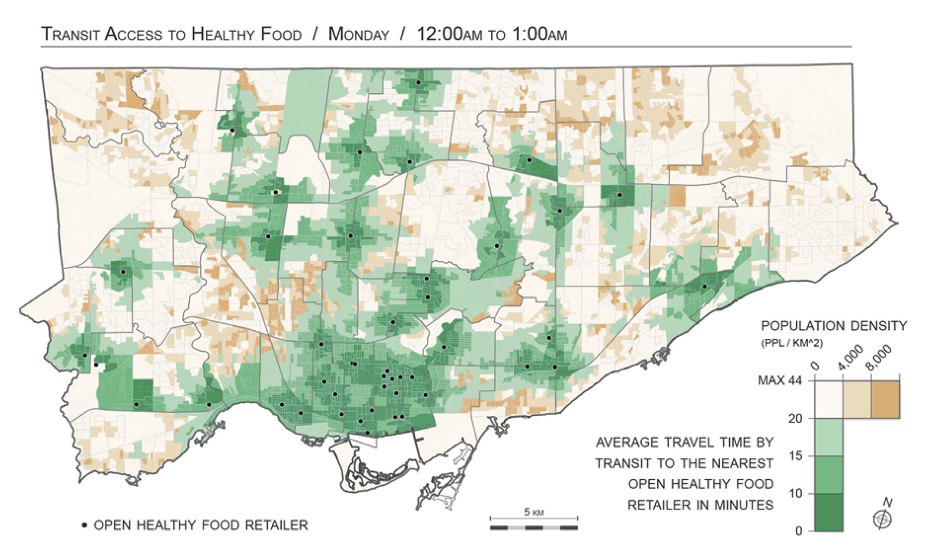
\includegraphics[width=0.94\linewidth]{images/food_midnight.png}
	\end{figure}
	
	\tiny Source: Widener et al (2017) How do changes in the daily food and transportation environments affect grocery store accessibility?
	\url{https://doi.org/10.1016/j.apgeog.2017.03.018}
	
\end{frame}




\begin{frame}
	
	\textbf{Accessibility, e.g. to food banks}
	
	\begin{figure}
		\centering
		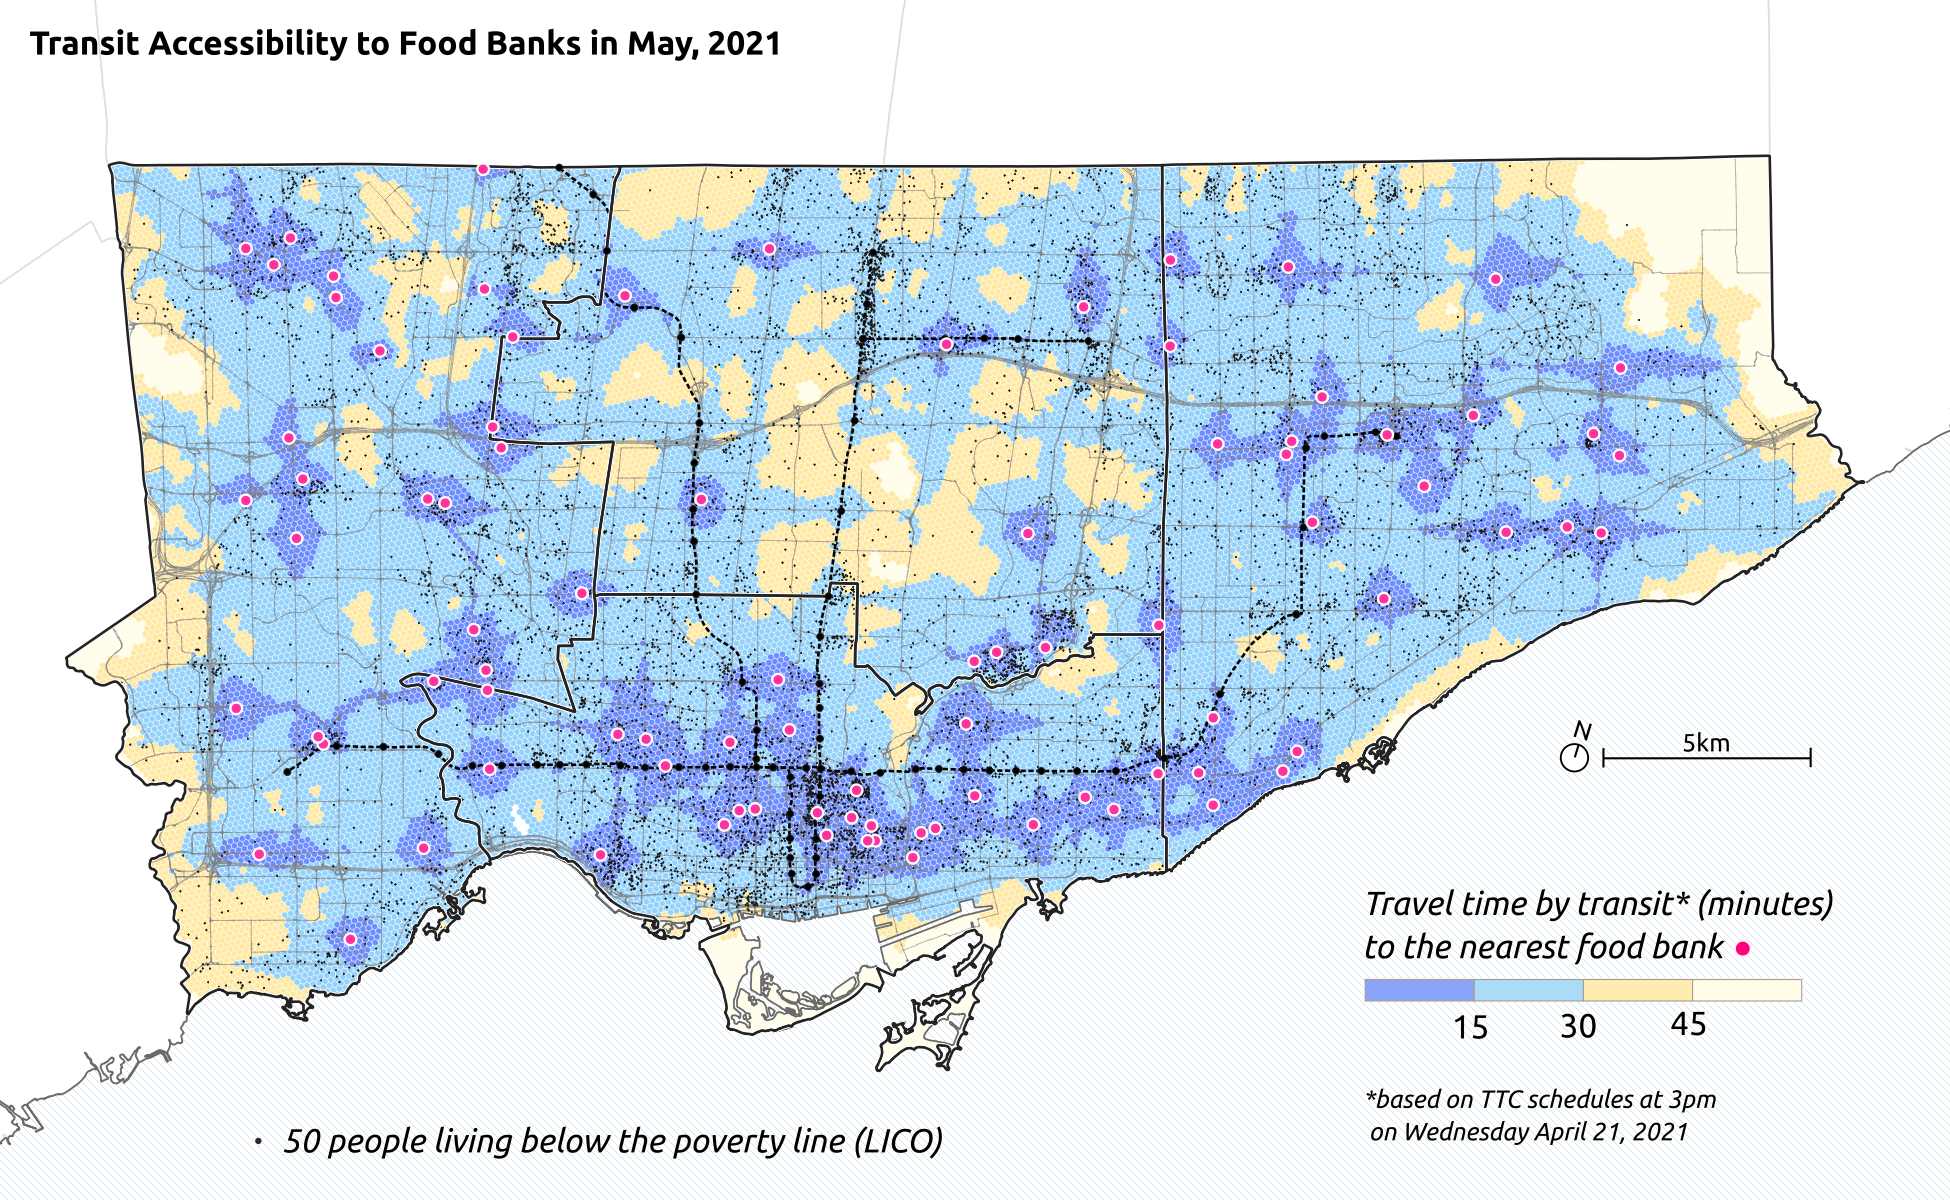
\includegraphics[width=0.94\linewidth]{images/foodbanks_access.png}
	\end{figure}
	
	\tiny 
	\url{https://github.com/SAUSy-Lab/toronto-food-bank-accessibility}
	
\end{frame}












\begin{frame}
	
	\textbf{Transport Equity}
	
	\vspace{4mm}
	
	
	\textit{Equity} generally refers to the fairness with which impacts (i.e. benefits and costs) are distributed 
	
	\vspace{2mm}
	
	Transportation planning decisions can have large and diverse equity
	impacts.
	
	\vspace{2mm}
	
	
	\begin{itemize}	
		\item \textbf{Horizontal Equity} - about the distribution of a resource (e.g. public transit) equally among the overall population
		
		\item \textbf{Vertical Equity} - about the distribution of a resource with focus towards specific groups, often those who are more vulnerable to social or economic exclusion
	\end{itemize}
	
	
\end{frame}




\begin{frame}
	
	\textbf{Transport Equity}
	
	\vspace{4mm}
	
	Dimensions of measuring transport equity
	
	\begin{itemize}	
		
		\item \textbf{Exposure} - about inequalities in exposure to pollutants, noise, crime, COVID-19 when travelling, etc.
		
		\item \textbf{Opportunities} - about how transportation infrastructure and accessibility are (in)equitably distributed
		
		\item \textbf{Outcomes} - about whether there are inequalities in travel behaviour outcomes, e.g. activity participation, commute times, etc.
		
	\end{itemize}
	
	
\end{frame}



\begin{frame}
	
	\begin{figure}
		\centering
		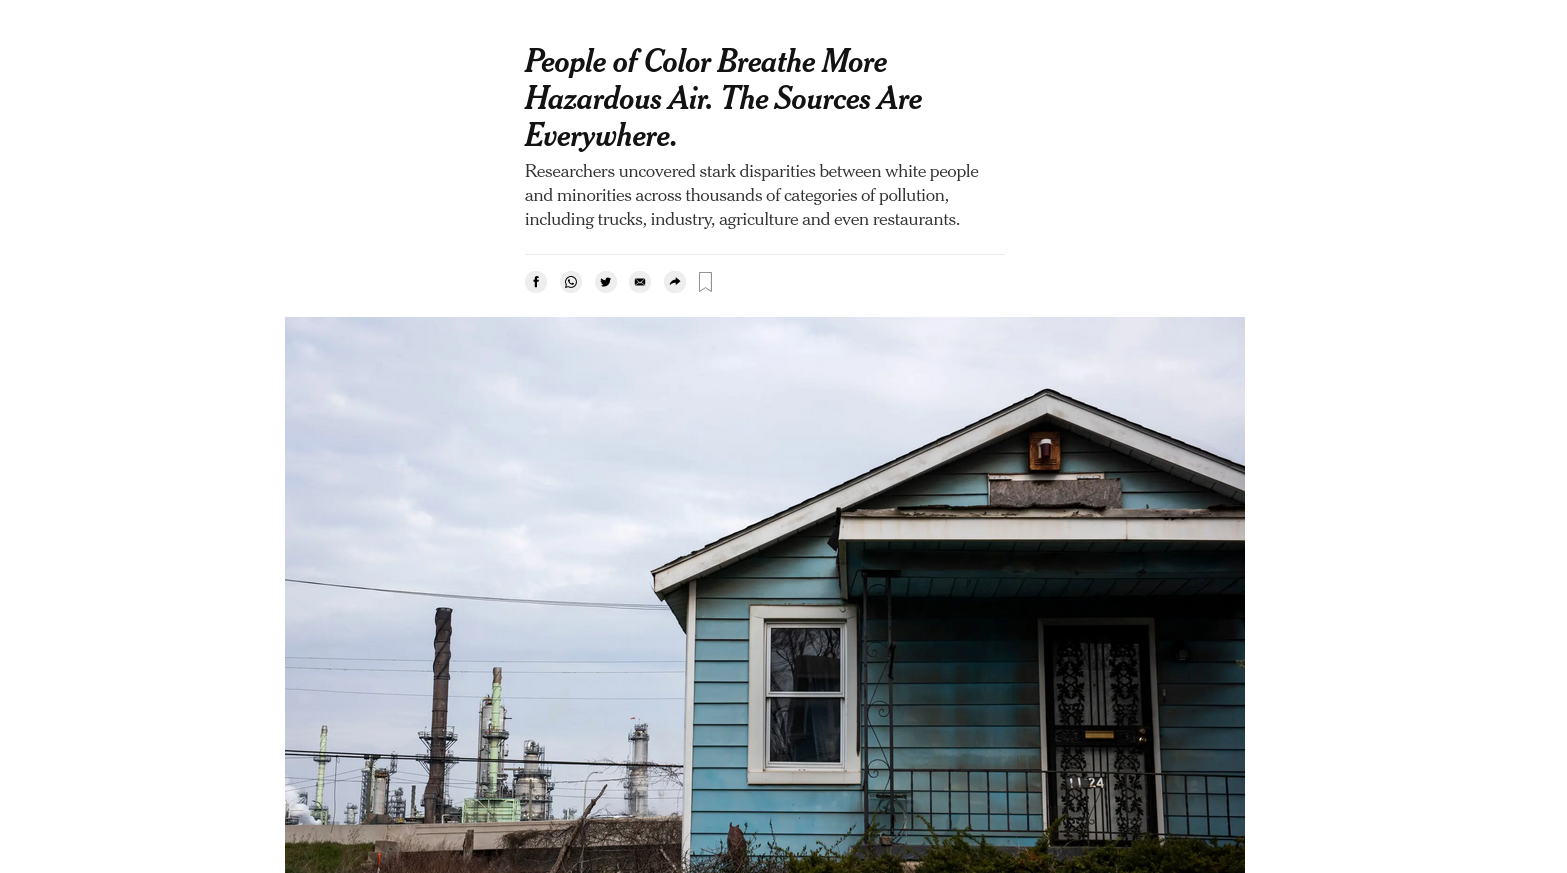
\includegraphics[width=1\linewidth]{images/race-pollution}
	\end{figure}

	\tiny\url{https://www.nytimes.com/2021/04/28/climate/air-pollution-minorities.html}
	
\end{frame}



\begin{frame}
	
	\begin{figure}
		\centering
		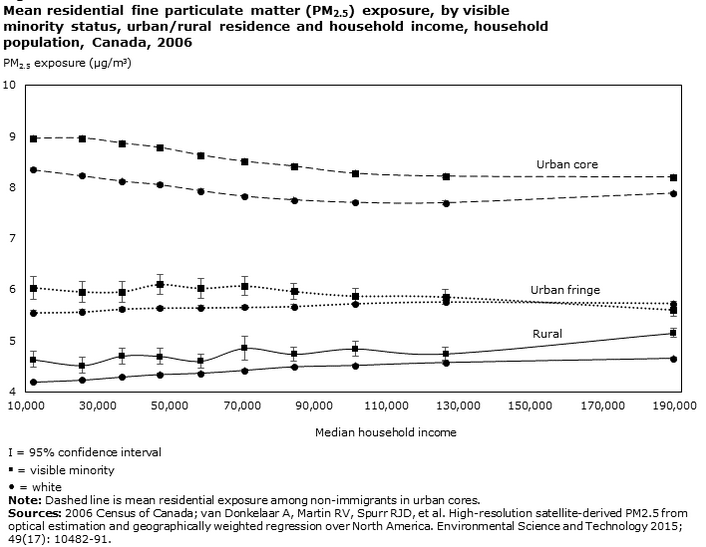
\includegraphics[width=0.8\linewidth]{images/race_pollution_canada.png}
	\end{figure}
	
	\tiny\url{https://www150.statcan.gc.ca/n1/pub/82-003-x/2017003/article/14781-eng.htm}
	
\end{frame}













\begin{frame}
	
	
	\textbf{Transit in Toronto}: Let's explore the connections between socioeconomic status and transit availability within the City of Toronto
	
	\vspace{2mm}
	
	
	\url{https://edu.maps.arcgis.com/apps/Cascade/index.html?appid=58618c037f344aaaada20b0c894e011c}
	
	
\end{frame}





\begin{frame}
	
	Income and mode share - for commuters across Canada
	
	\begin{figure}
		\centering
		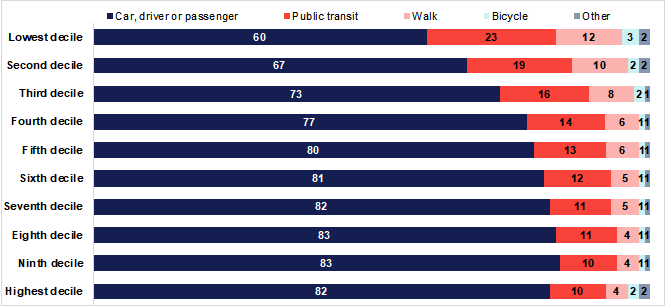
\includegraphics[width=0.94\linewidth]{images/income_mode_canada.png}
	\end{figure}
	
	\tiny\url{https://mobilizingjustice.ca/how-the-canadian-population-gets-to-work/}
	
\end{frame}





\begin{frame}
	
	\begin{figure}
		\centering
		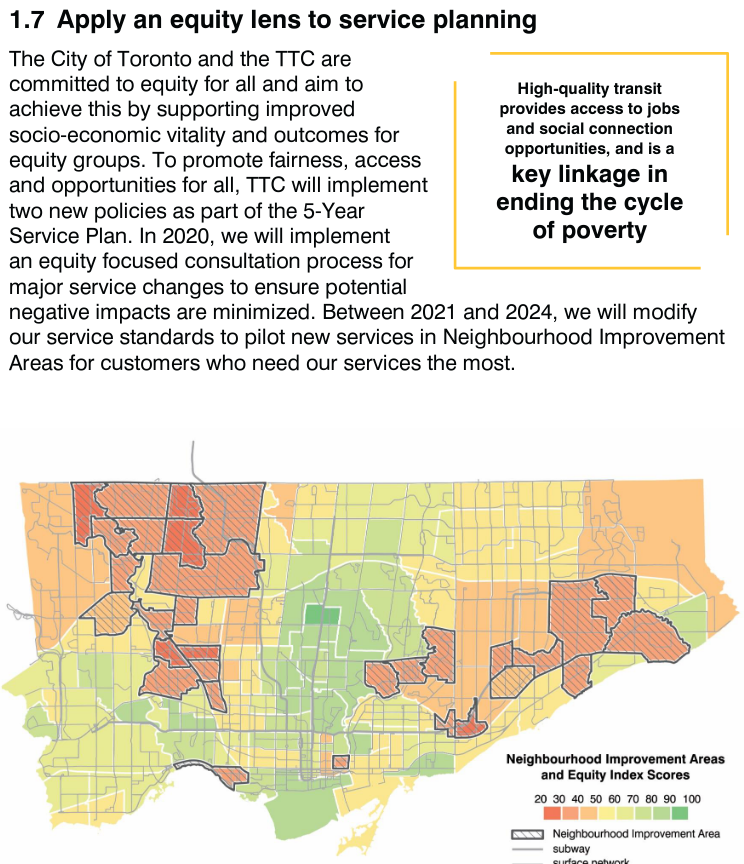
\includegraphics[width=0.5\linewidth]{images/ttc_equity.png}
	\end{figure}
	
	\tiny\url{https://www.ttc.ca/about-the-ttc/projects-and-plans/5-Year-Service-Plan-and-10-Year-Outlook}
	
\end{frame}







\begin{frame}
	
	Accessibility and income - for neighbourhoods across Canada
	
	\begin{figure}
		\centering
		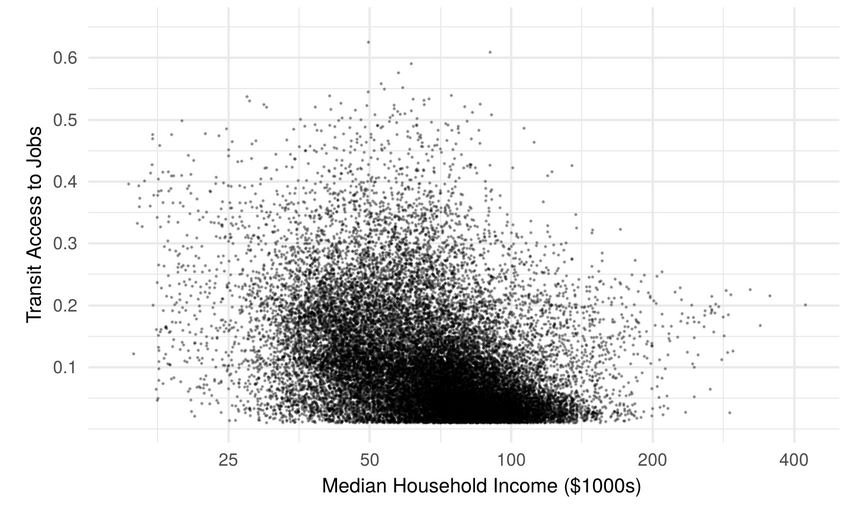
\includegraphics[width=0.94\linewidth]{images/access_income.png}
	\end{figure}
	
	\tiny\url{https://doi.org/10.1016/j.tranpol.2018.11.018}
	
\end{frame}



\begin{frame}
	
	Accessibility and income - counting by city
	
	\begin{figure}
		\centering
		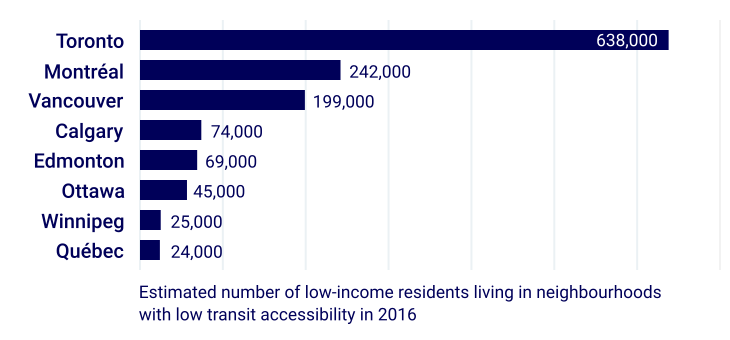
\includegraphics[width=0.74\linewidth]{images/tpov_city_plot.png}
	\end{figure}

	\tiny\url{https://doi.org/10.1016/j.tranpol.2018.11.018}
	
\end{frame}




\begin{frame}
	
	Accessibility and income - for individuals in the GTHA
	
	\begin{figure}
		\centering
		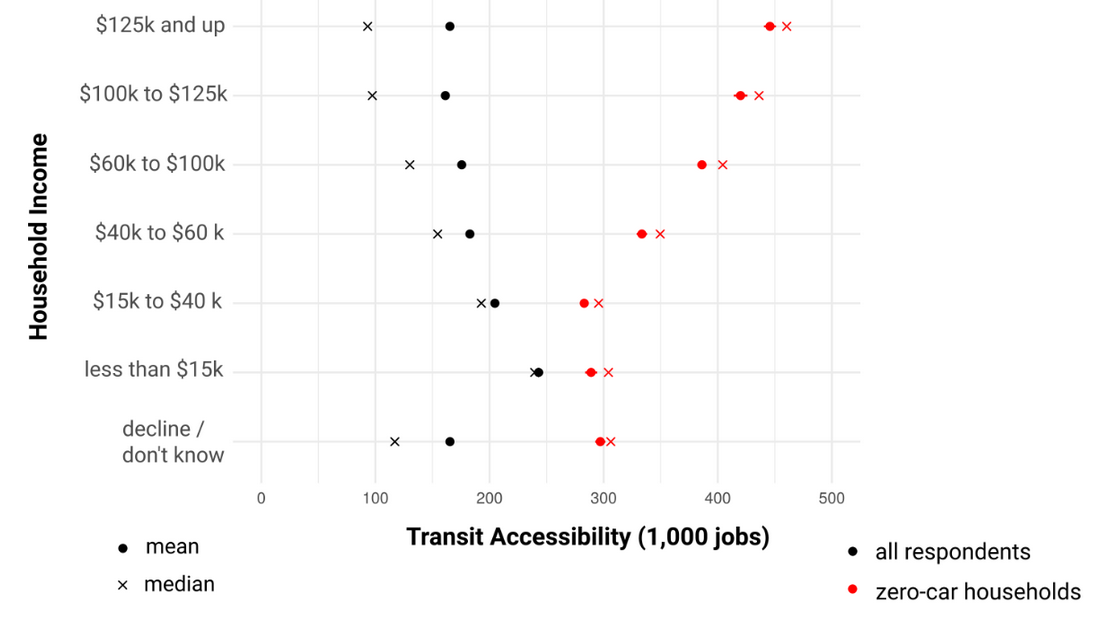
\includegraphics[width=0.94\linewidth]{images/income_transit_gtha.png}
	\end{figure}
	
\end{frame}



\begin{frame}
	
	\textbf{Spatial Mismatch}
	
	\begin{itemize}
		\item The mismatch between where low income households live and
		where suitable job opportunities are available
		
		\item Originally pertained to low-income inner-city Americans
		were socioeconomically excluded from living in suburbs,
		coupled with the movement of both manufacturing and retail
		sectors to the suburbs
		
		
		\begin{itemize}
			\item suburban employment is far away
			\item lack of car + poor transit to the suburban employment
		\end{itemize}
	\end{itemize}
	
\end{frame}




\begin{frame}
	
	\begin{figure}
		\centering
		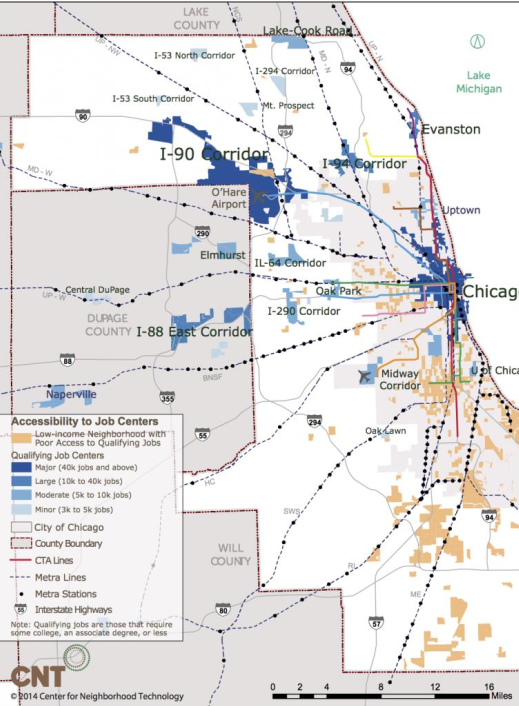
\includegraphics[width=0.48\linewidth]{images/chicago_spatial_mismatch.png}
	\end{figure}
	
\end{frame}



\begin{frame}
	
	\begin{figure}
		\centering
		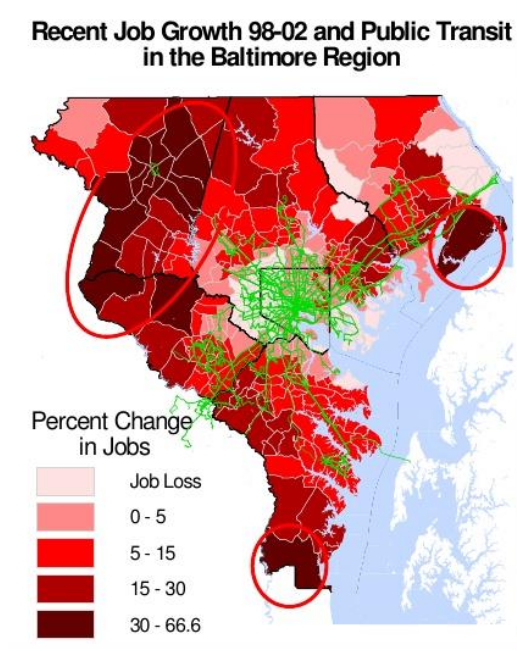
\includegraphics[width=0.54\linewidth]{images/baltimore_spatial_mismatch.png}
	\end{figure}
	
\end{frame}





\begin{frame}
	
	\begin{figure}
		\centering
		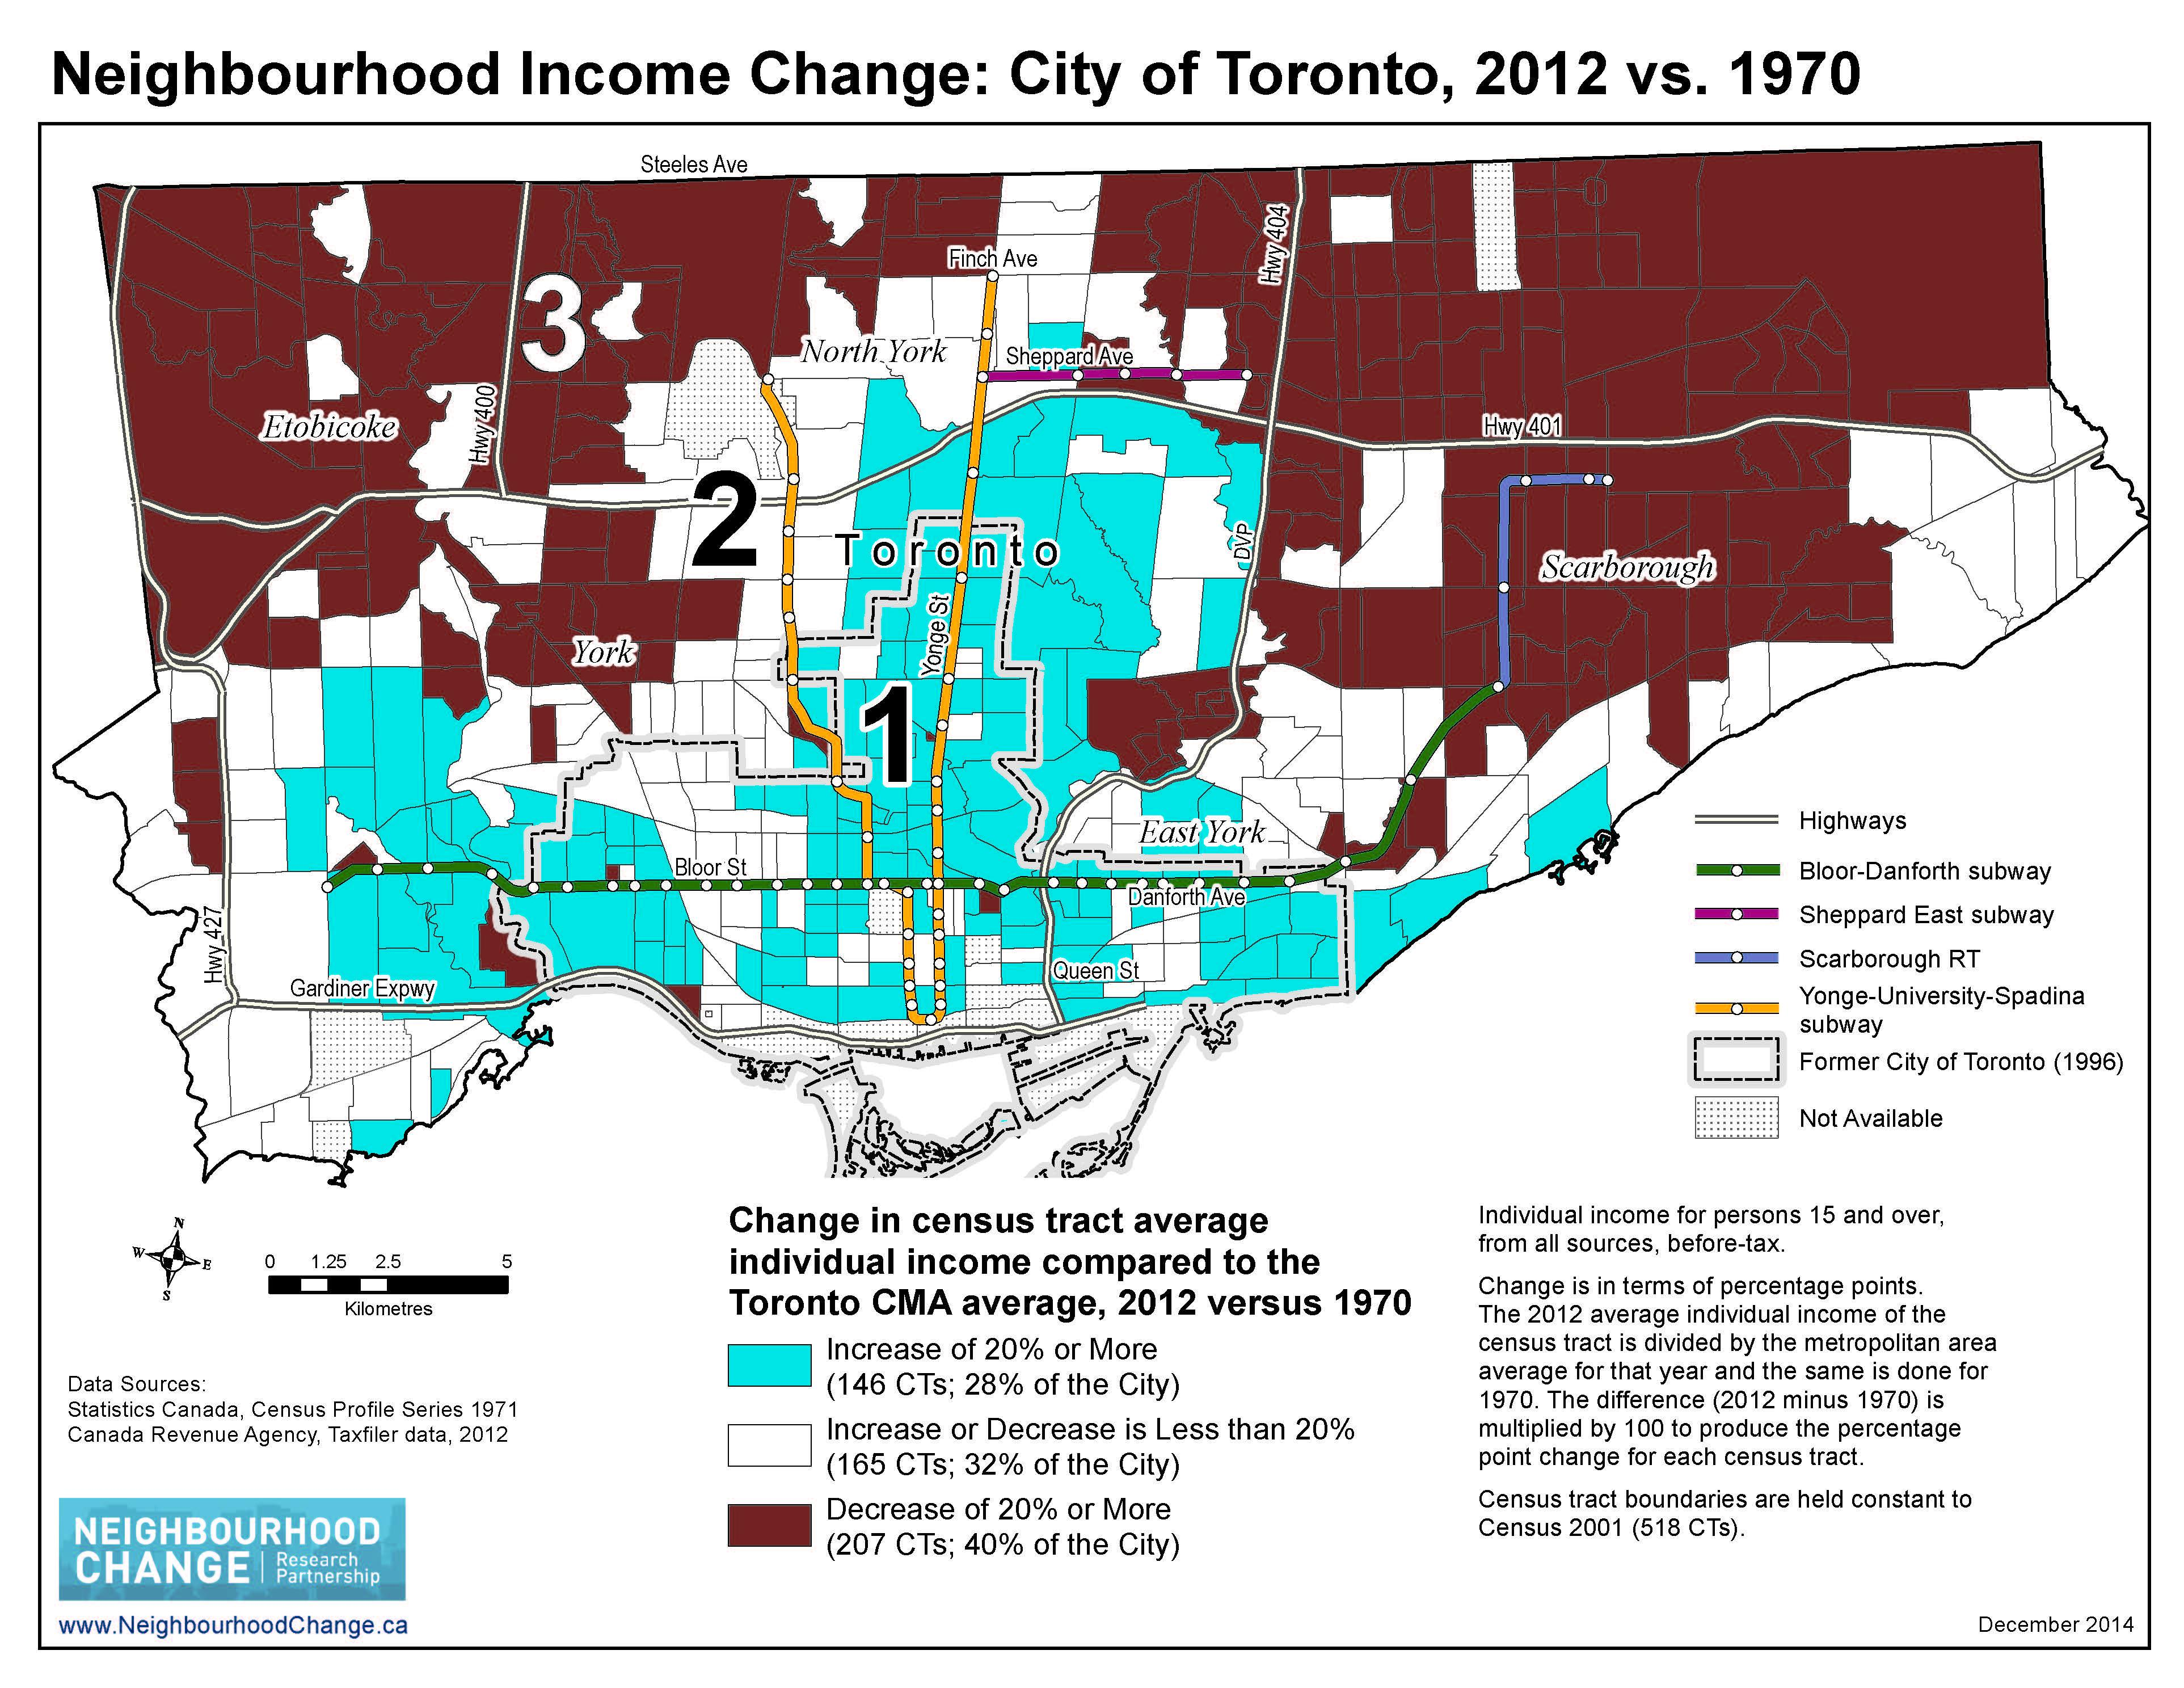
\includegraphics[width=0.84\linewidth]{images/3cities_2012_1970.jpeg}
	\end{figure}
	
\end{frame}




\begin{frame}
	
	Cycling infrastructure and neighbourhood-level income in Canada
	
	\begin{figure}
		\centering
		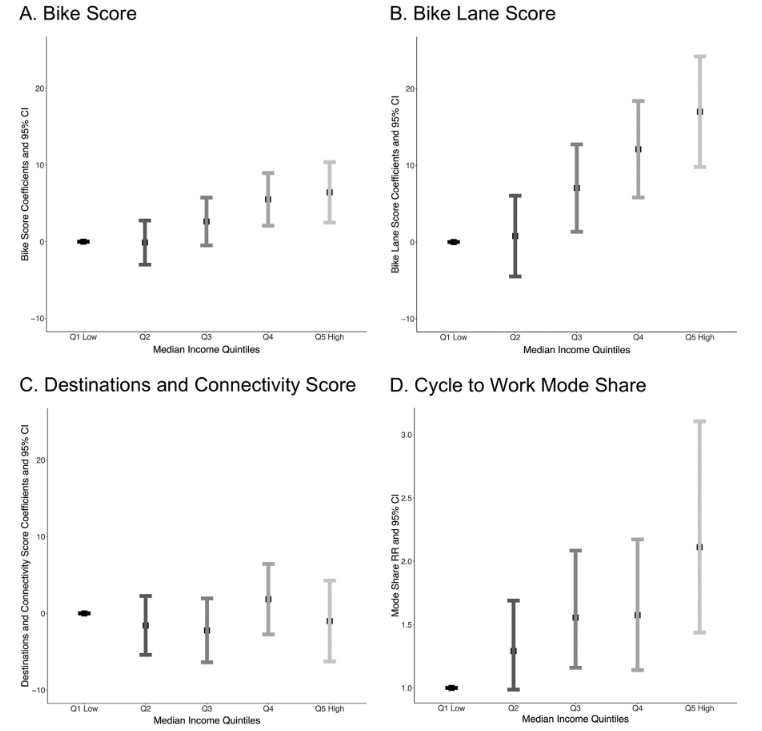
\includegraphics[width=0.6\linewidth]{images/bikescore_income.png}
	\end{figure}
	
	\tiny Income inequalities in Bike Score and bicycling to work in Canada \url{https://doi.org/10.1016/j.jth.2017.09.005}
	
\end{frame}





\begin{frame}
	
	What are the impacts of a new transit line on social equity?
	
	
	\begin{figure}
		\centering
		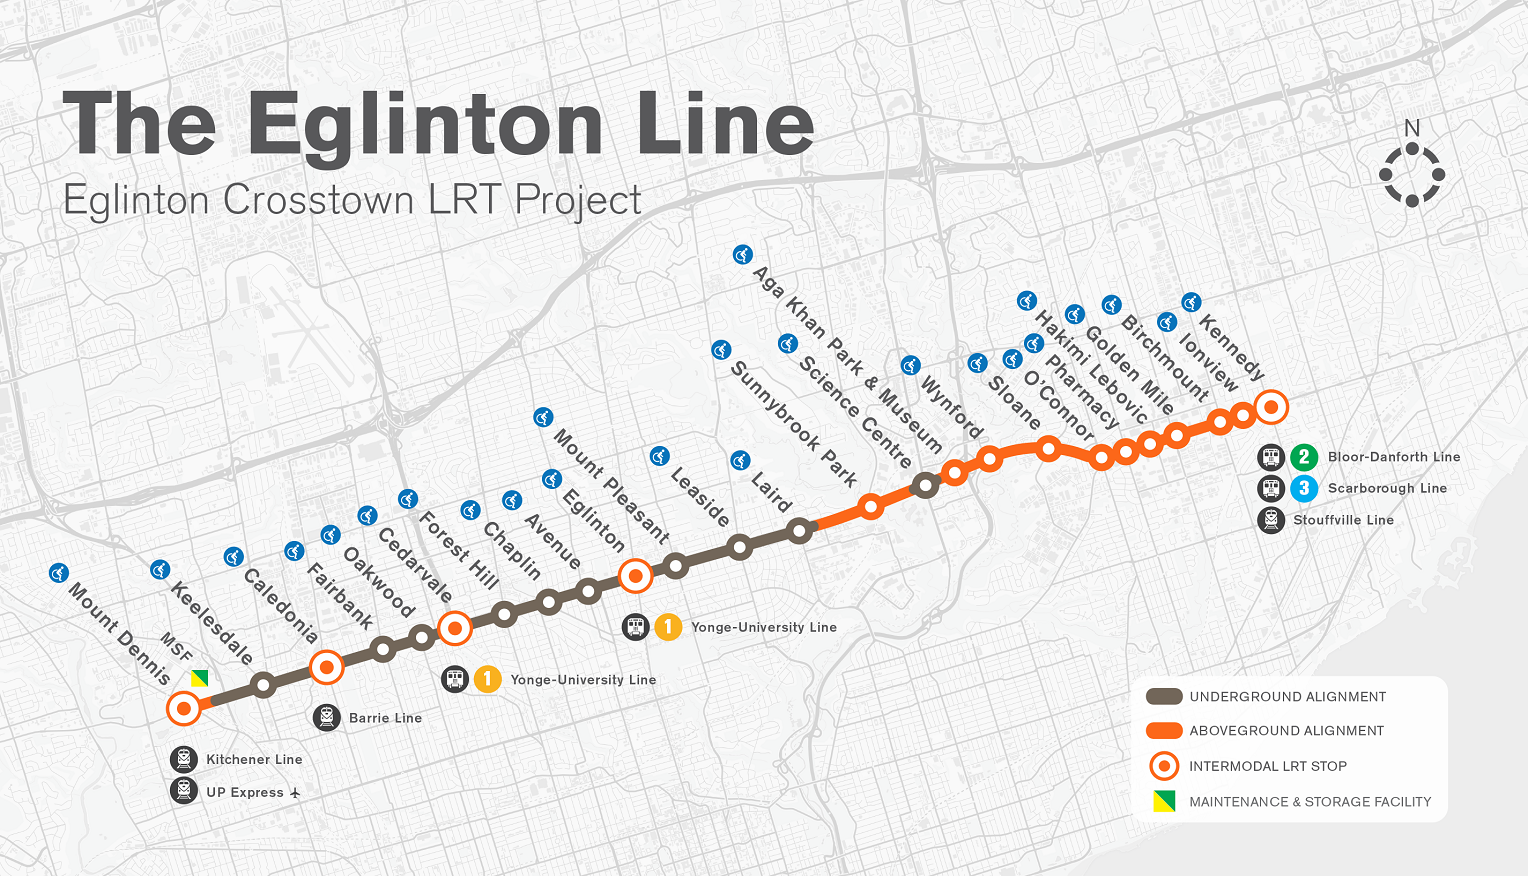
\includegraphics[width=0.74\linewidth]{images/crosstown.png}
	\end{figure}
	
	
\end{frame}



\begin{frame}
	
	\textbf{Transport and Social Exclusion}
	
	“the process by which people are prevented from
	participating in the economic, political, and social
	life of the community because of reduced
	accessibility to opportunities, services and social
	networks, due in whole or in part to insufficient
	mobility in a society and environment built around
	the assumption of high mobility” Kenyon et al. (2003:210)
	
\end{frame}






\begin{frame}
	
	\textbf{Transport Poverty \& Social Exclusion}
	
	\begin{figure}
		\centering
		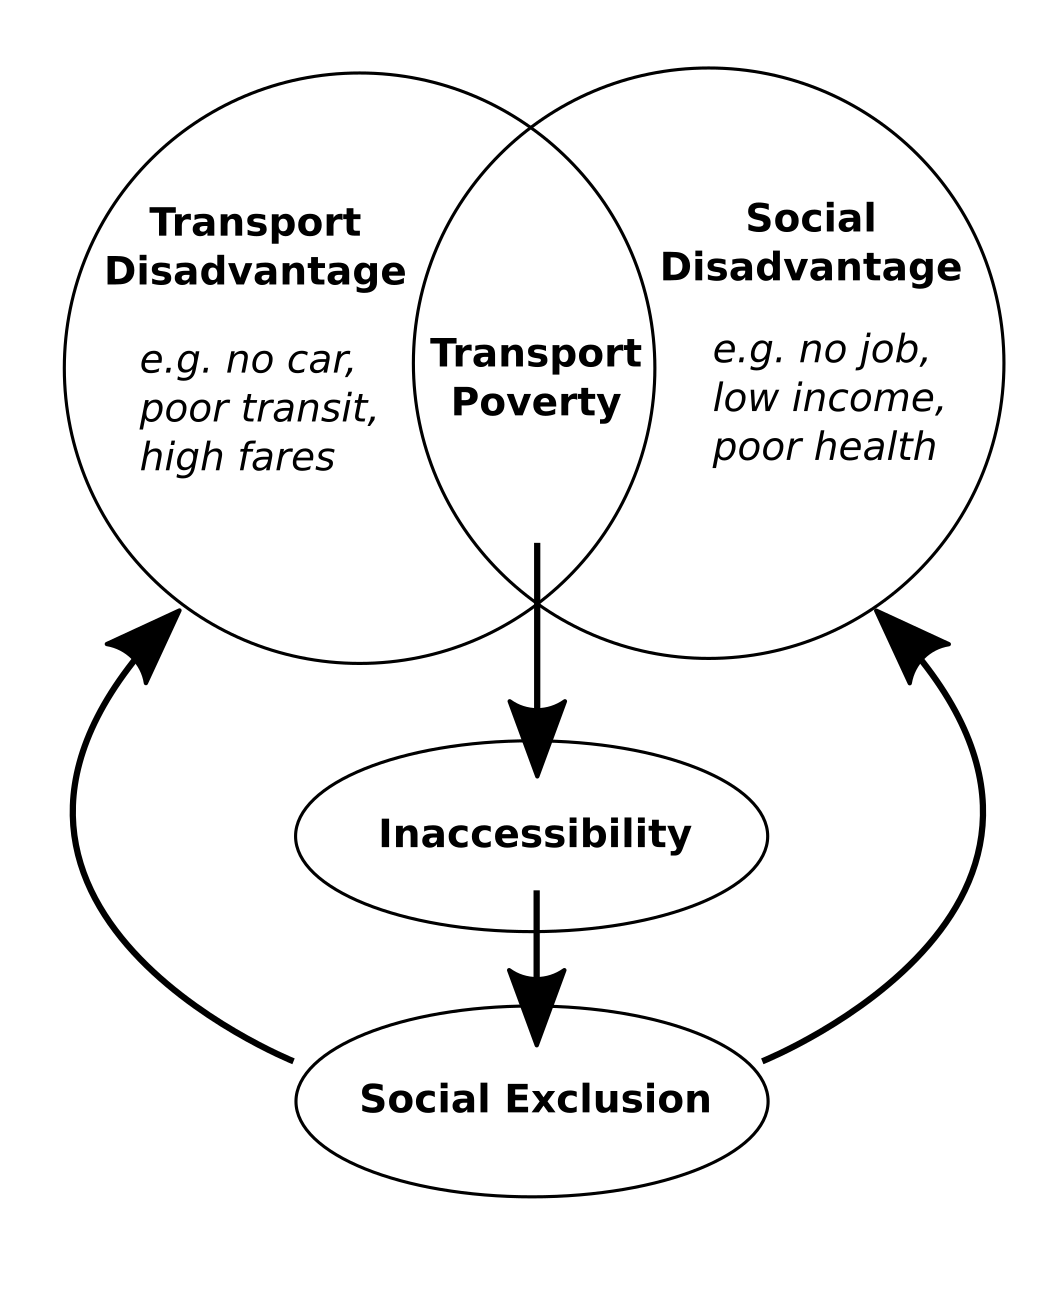
\includegraphics[width=0.44\linewidth]{images/tpov.png}
	\end{figure}
	
	\tiny Figure adapted from Lucas (2012) Transport \& Social Exclusion: Where are we now
	
\end{frame}




\begin{frame}
	
	Income and activity participation - for individuals in the GTHA
	
	\begin{figure}
		\centering
		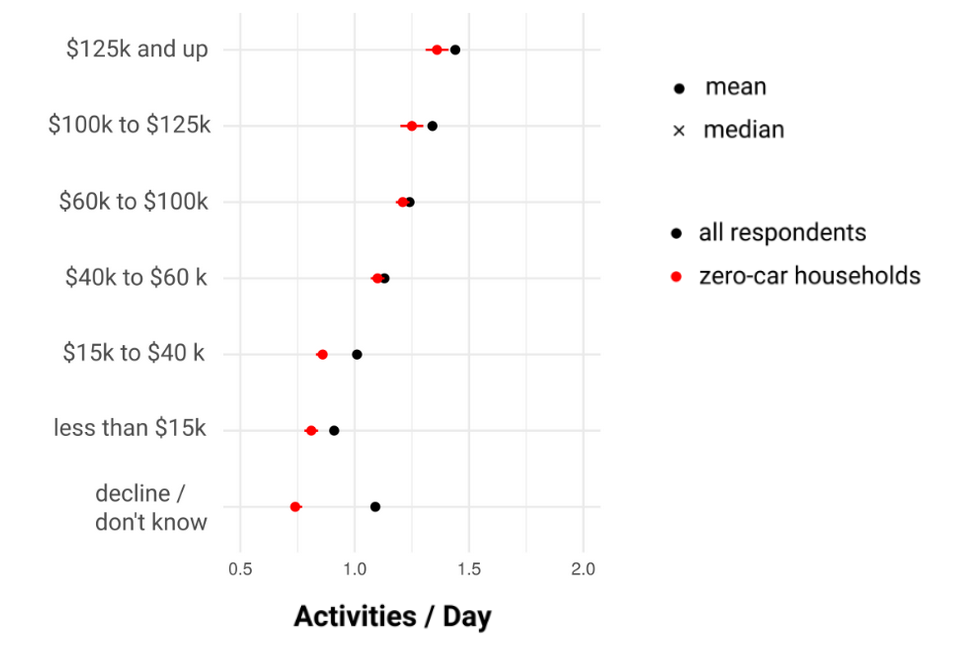
\includegraphics[width=0.94\linewidth]{images/income_activities_gtha.png}
	\end{figure}
	
\end{frame}




\begin{frame}
	
	Accessibility and activity participation - for individuals in the GTHA
	
	\begin{figure}
		\centering
		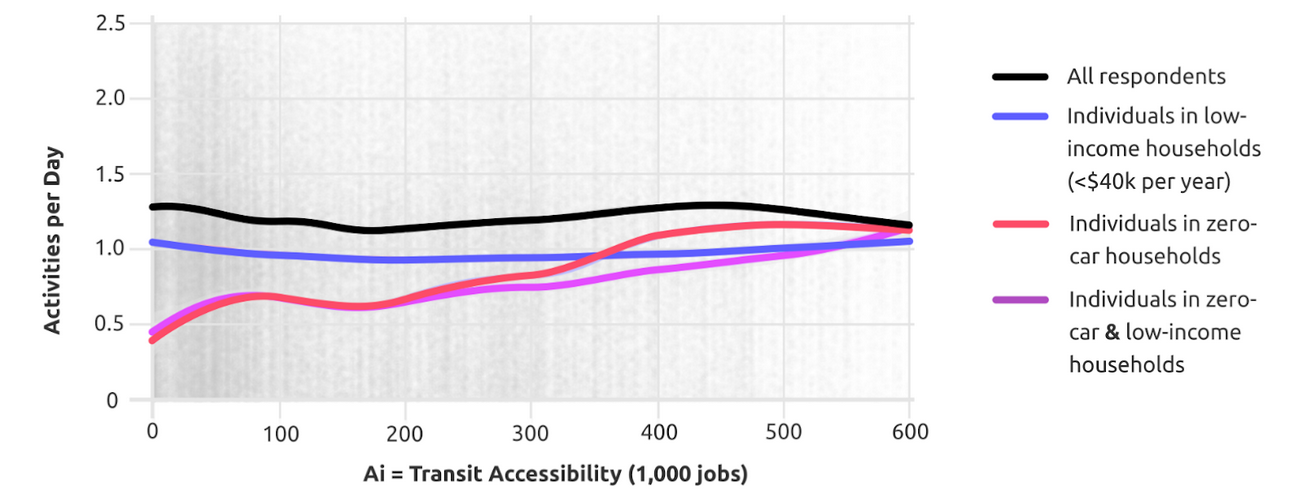
\includegraphics[width=0.94\linewidth]{images/accessibility_activities_gtha.png}
	\end{figure}
	
\end{frame}





\begin{frame}
	
	Benefits of cars for alleviating (transport) poverty
	
	\begin{figure}
		\centering
		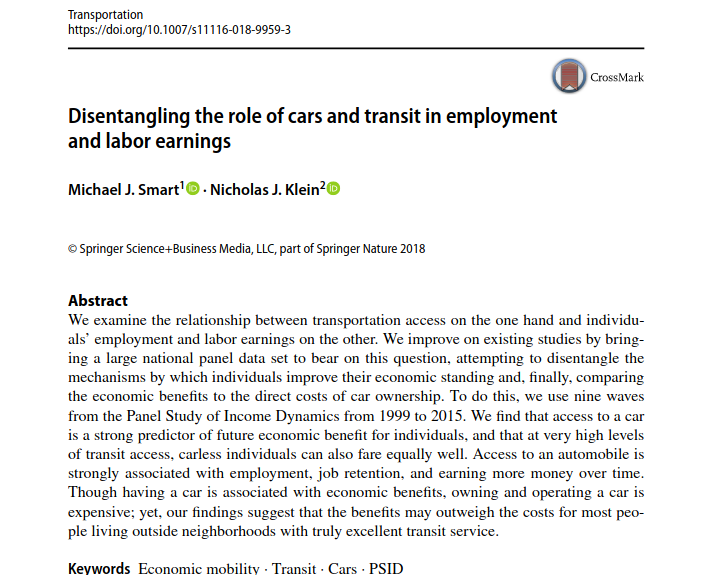
\includegraphics[width=0.64\linewidth]{images/klein_smart_cars.png}
	\end{figure}

	\tiny\url{https://link.springer.com/article/10.1007/s11116-018-9959-3}
	
\end{frame}


%Physical exclusion inhibiting use of transport services
%
%Geographical exclusion of residence
%
%Geographical exclusion of destinations
%
%Economic exclusion (i.e. affordability of mobility)
%
%Time-based exclusion (i.e. time poverty) where competing
%home and work demands on time make travel inaccessible
%
%6. Fear-based exclusion when fear for personal safety inhibits use
%of transport services
%
%7. Space exclusion, where security or space management inhibit
%use of public spaces (e.g. malls and gated communities)





\begin{frame}
	
	\textbf{Discussion Question:}
	
	\vspace{2mm}
	
	Should the government provide subsidies for low-income households to purchase/lease cars in the suburbs of the GTHA?
	
\end{frame}





\end{document}